% ============================================================
%  Chapter fragment -- included by main.tex
%  (not a standalone document; compile main.tex to build the PDF)
% ============================================================
\begin{multicols*}{3}
\raggedcolumns

\sheettitle{02 -- Threat Landscape}{SWS2 -- ZHAW / Tellenbach}

% ==================== CHAPTER 2: THREAT LANDSCAPE ====================
\section{Threat Landscape -- Basics}

\subsection{Definition}
A collection of \kw{threats, threat actors (agents)} and \kw{observed trends}. Tracking it = knowing:
\begin{itemize}
\item threat agents \& their \kw{capabilities}
\item \kw{weapons} and \kw{tactics} used
\item which threats are \kw{most relevant}
\item \kw{emerging} threats \& actors
\end{itemize}
\textbf{Why:} know your enemy / prepare; motivates \kw{investment} in controls.

\subsection{Elements of Risk (relationship)}
\kw{Threat agents} use \kw{attack vectors} $\to$ give rise to \kw{threats} that exploit \kw{vulnerabilities} $\to$ lead to \kw{risks} to \kw{assets}. Owners impose \kw{countermeasures} to reduce risk. Threat Landscape = threat agents + attack vectors + threats.

\begin{center}
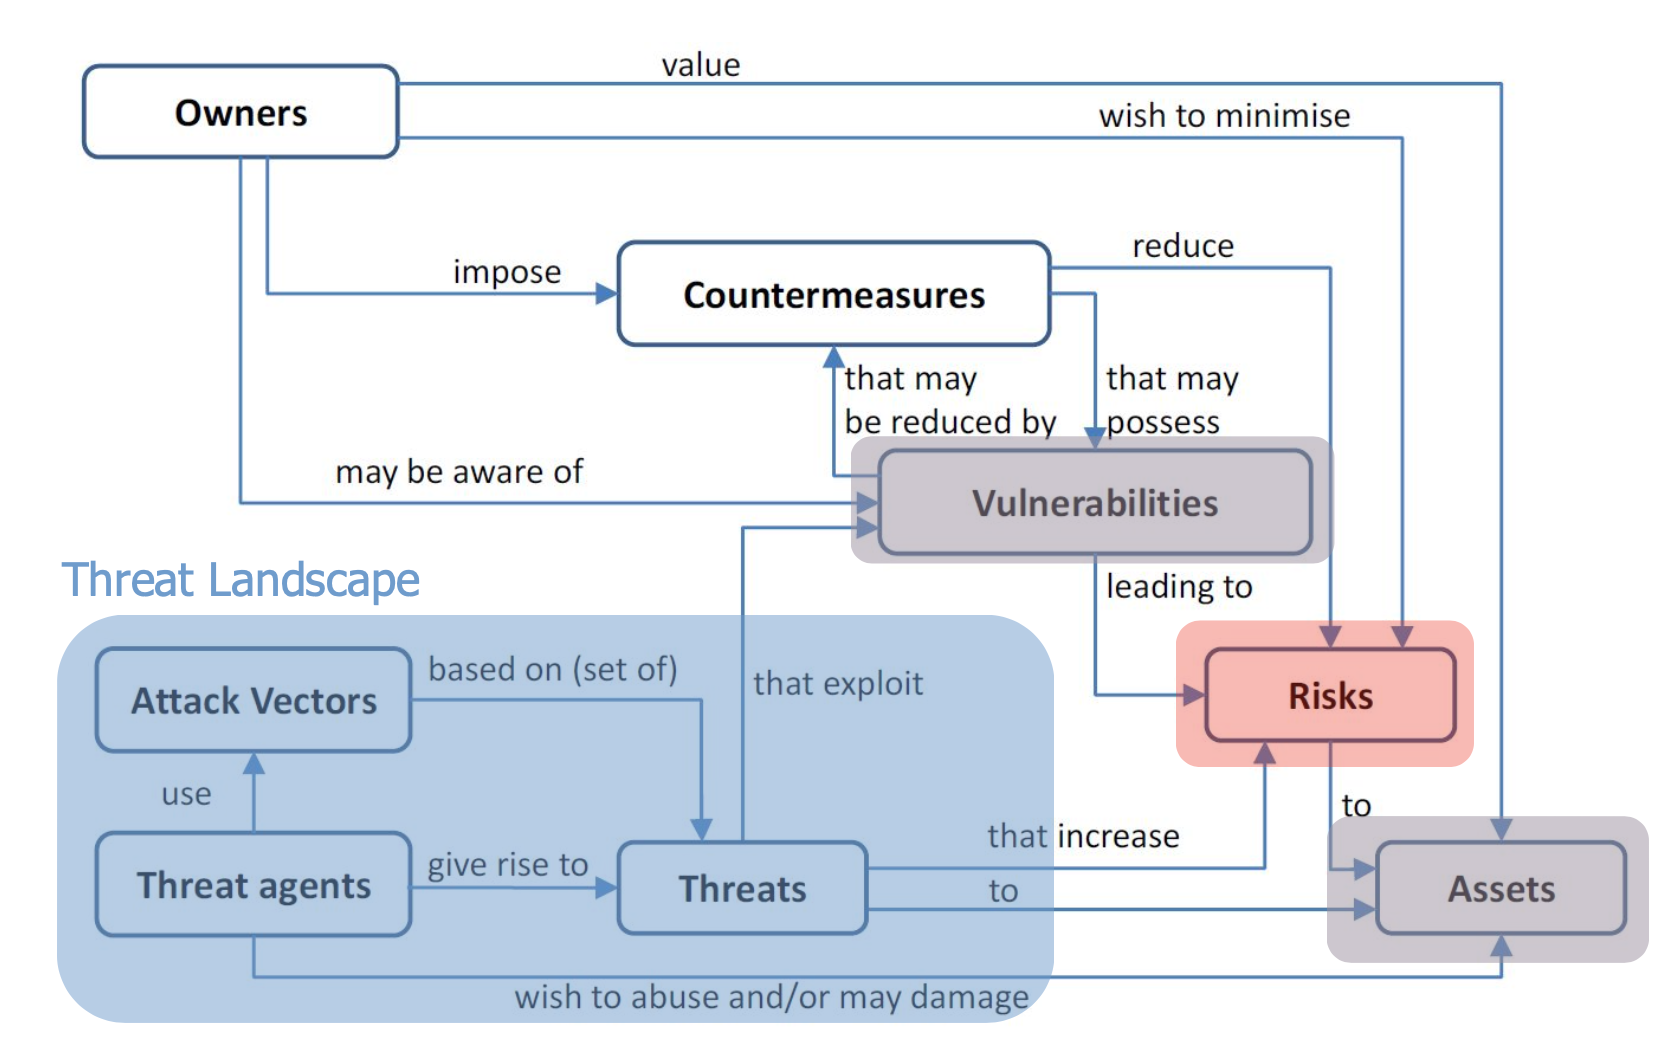
\includegraphics[width=\linewidth]{Figures/threat_landscape.png}
\end{center}

\subsection{Importance for Risk}
\kw{Risk = Likelihood $\times$ Impact}; Risk = Threat $\times$ Vulnerability $\times$ Consequence. The threat landscape is \kw{external / out of your hands} and drives the likelihood part.

\subsection{Important Elements}
\begin{itemize}
\item \kw{Threat actors}: state actors, cyber criminals, insiders... Attributes: \kw{motivation, skill/resources, organization, tactics}.
\item \kw{Threats}: type+description (ransomware, phishing...), \kw{targeted assets}, \kw{attack vectors} (methods/tools, split in phases $\to$ kill chain).
\end{itemize}
\textit{No standardized way} to characterize; lines between actors/types often \kw{blurred}; companies define own vocabulary.

% ==================== THREAT ACTORS ====================
\section{Threat Actors}

\subsection{Profile parameters}
\kw{Motivation} (intel/money/destruction/fame), \kw{Resources} (low/med/high), \kw{Skill} (low/med/high), \kw{Role}: Developer / Provider / Operator / User (\kw{Dev/Pro/Op/User}).

\subsection{Cybercrime}
\begin{itemize}
\item \kw{Profit} from illegal activity; optimize \kw{ROI} (max money / min effort+risk). Mot: Money; Res: Med--High; Skill: Low--High; Roles: User+Dev/Prov/Op.
\item \kw{Professionalized industry} -- division of labor via \kw{*-as-a-Service} (below).
\item \kw{Ransomware} (top tactic) -- extortion levels:
  \begin{itemize}
  \item \kw{Single}: encrypt data, sell decryption key (backups defeat it).
  \item \kw{Double}: also \kw{exfiltrate} \& threaten to leak (backups don't save you).
  \item \kw{Triple}: + DDoS / pressure customers \& partners.
  \end{itemize}
\item Delivery: \kw{automated} (masses) vs \kw{human-operated = Big Game Hunting} (high-value targets).
\item Other tactics: \kw{social engineering}, exploit \kw{WFH/remote access}, low-hanging fruit (SMEs, bad cloud), attack \kw{MSPs} (1 hit $\to$ all their customers).
\item Challenges: \kw{cross-border} (diff. legal frameworks), takedowns not sustainable (infra disposable).
\item \term{Ex: DarkSide RaaS / Colonial Pipeline (2021)} -- billing crippled $\to$ 6-day shutdown, fuel shortage, \$5M BTC; FBI recovered 63.7 BTC.
\end{itemize}

\subsection{*-as-a-Service ("anything"-aaS)}
Attack capabilities \kw{packaged \& rented} like cloud products (SaaS-style) $\Rightarrow$ \kw{lowers barrier to entry} (no skill needed, just buy). Often w/ updates, \kw{AV evasion}, support, SLAs.
\begin{itemize}
\item \kw{Roles}: Developer (builds) / Provider (infra/access) / Operator (runs) / User (buys \& aims).
\item Types: \kw{RaaS} (ransomware), \kw{AaaS} (access), \kw{PaaS} (phishing), + infection/spam/DDoS.
\end{itemize}
\textit{Prices:} {\scriptsize \$8 iTunes creds \textbullet{} \$40 20k spam \textbullet{} \$100 infection 1k installs \textbullet{} \$1000 DDoS 1 month \textbullet{} \$40k malware+bootkit \textbullet{} \$400k+ GovWare}

\subsection{Nation States / State-Sponsored}
\begin{itemize}
\item Act in interest of a state, in \kw{secret}. Mot: strategic (espionage); Res: High; Skill: High; Roles: User+Dev/Op.
\item Targets: state/military secrets, critical infrastructure.
\item Tactics: \kw{long-term, novel, sophisticated} -- zero-days, \kw{APT}, supply chain, ICS, AI, hack-and-leak.
\item Trend: also act for \kw{personal gain} (blurs espionage/crime).
\item Challenges: legal for them; \kw{sanctions \& name-and-shame}; use \kw{false flags} \& standard tools.
\item \term{Ex: SolarWinds (SUNBURST)} -- trojanized Orion updates, supply-chain, attrib. Russia (APT29), discovered by FireEye 12/2020.
\end{itemize}

\subsection{Hacker-for-Hire}
\begin{itemize}
\item Companies offering \kw{offensive cyber capabilities} (vuln research, exploitation, malware, C2, mgmt, support). Mot: Work/Job; Res: High; Skill: Professionals; Roles: Dev/Pro/Op.
\item Bundled services: AaaS, RaaS, PaaS.
\item Clients usually governments $\to$ \kw{plausible deniability} (proxy).
\item Operate \kw{legally} in their country; hard to predict.
\item \term{Ex: NSO Group / Pegasus spyware} -- SMS links, network injection, \kw{zero-click}; spies on journalists/critics; lawsuits (WhatsApp).
\end{itemize}

\subsection{Hacktivist}
\begin{itemize}
\item Individuals/loose groups (e.g. Anonymous) for \kw{social/political change}. Mot: Work; Res: Low*; Skill: Low--Med; Roles: User.
\item Tactics \kw{old school}: \kw{(D)DoS}, \kw{defacements}, release sensitive data.
\item Hard to predict -- \kw{event-driven}; crowd-sourcing = huge leverage.
\item \term{Ex: Tillie Kottmann / APT 69420} -- Verkada hack (150k cams) via exposed creds, Google dorking.
\end{itemize}

\subsection{Insider}
\begin{itemize}
\item \kw{Unintentional} (lax procedures $\to$ address w/ \kw{DLP}) or \kw{intentional} (steal/leak/sabotage). Mot: extortion/revenge/profit; Res: Low; Skill: Low--Med; Roles: User.
\item Challenge: \kw{legitimate access} + know the protections.
\item Important: spot unhappy employees, close knowledge gaps, monitor unusual activity, limit access.
\end{itemize}

\subsection{Others}
\begin{itemize}
\item \kw{Script Kiddy}: runs tools without knowing; *-aaS boosts activity. (\textit{Can do SQLi via tools -- yes.})
\item \kw{Cyber Terrorists}: disruption for alarm/panic; no commonly accepted definition; no major event yet.
\end{itemize}

% ==================== THREATS ====================
\section{Threats}

\subsection{Knowing threats -- why?}
Roadmap for future (policy/biz/research); learn new attack vectors. Helps \kw{CEO/CIO} (risks to business), \kw{CISO} (trainings, new/modified controls), \kw{SecOps} (patterns, indicators).

\subsection{Threat Taxonomy}
\kw{Classification of threat types} at various detail $\to$ common language. Many proposals (no one-fits-all): \term{Open Threat Taxonomy, ENISA, NIST, Operational Cyber Sec Risks, Cambridge Risk Framework}.
\textit{Open Threat Taxonomy categories:} Physical, Resource, Personnel, Technical threats (w/ threat rating).

% ==================== SOURCES ====================
\section{Sources of Information}

\subsection{Long term (strategic/tactical)}
Threat reports few times/year: \kw{ENISA ETL}, Fortinet, Bitdefender, Proofpoint, McAfee. Some describe threats only (not whole landscape).

\subsection{Short term ("real-time")}
\begin{itemize}
\item News portals (Heise Security, DarkReading), security mailing lists.
\item \kw{Threat intelligence providers}: advisories + \kw{actionable info} (CERTs, OTX feed), real-time web pages.
\item \kw{Threat Intelligence Platforms}: aggregate/correlate, \kw{machine-readable} data $\to$ IDS/IPS/SIEM.
\item Exchange formats: \kw{STIX} (Structured Threat Info Expression), \kw{TAXII} (Trusted Automated eXchange of Indicator Info).
\end{itemize}

% ==================== APT & KILL CHAIN ====================
\section{APT \& Cyber Kill Chain}

\subsection{Advanced Persistent Threat \hl{(!)}}
\begin{itemize}
\item \kw{Advanced}: advanced tech/techniques to penetrate defenses (own/unknown vulns); develop tools as needed.
\item \kw{Persistent}: maintain \kw{long-term} access, keep trying, \kw{hide} from detection until objective reached.
\item \kw{Threat}: coordinated \kw{human} actions; skilled, motivated, organized, well-funded with a specific objective.
\item Bad: median \kw{243 days} attacker present before detection.
\end{itemize}

\subsection{Cyber Kill Chain (Lockheed Martin) \hl{(!)}}
Identifies what adversary must complete; \kw{intrusion-centric} (not all attacks fit). \kw{Defender advantage}: attack succeeds only if all steps succeed $\to$ defenders disrupt at \kw{any} step.

\textbf{Preparation:}
\begin{itemize}
\item \kw{1 Reconnaissance}: gather public info on target.
\item \kw{2 Weaponization}: build exploit + malicious payload.
\end{itemize}
\textbf{Intrusion:}
\begin{itemize}
\item \kw{3 Delivery}: send payload (email/USB/web).
\item \kw{4 Exploitation}: exploit vuln to execute payload.
\item \kw{5 Installation}: install malware (can be in-memory).
\end{itemize}
\textbf{Active Breach:}
\begin{itemize}
\item \kw{6 Command \& Control (C2)}: remote channel (generic, throughout attack).
\item \kw{7 Action on Objectives}: achieve goals inside network (months, 100s of steps).
\end{itemize}

\subsection{Summary}
\begin{itemize}
\item Many threat agents, different motivations/tactics/skill/resources/roles.
\item Orgs must consider which agents are \kw{most relevant}.
\item Kill chain $\to$ kill attack at any step; APT $\Rightarrow$ you're hacked.
\item \hl{Not a fair game}: attacker finds \kw{one} hole, defender must fix \kw{all}.
\end{itemize}

\end{multicols*}
